%%%%%%%%%%%%%%%%%%%%%%%%%%%%%%%%%%%%%%%%%%%%%%%%%%%%%%%%
\fondo{celeste}
\section{Redes convolucionales}
\fondo{blanco}
%%%%%%%%%%%%%%%%%%%%%%%%%%%%%%%%%%%%%%%%%%%%%%%%%%%%%%%%


%%%%%%%%%%%%%%%%%%%%%%%%%%%%%%%%%%%%%%%%%%%%%%%%%%%%%%%%
\begin{frame}
    \frametitle{Redes convolucionales}

    \begin{itemize}
        \item Se inspiran en la corteza visual de los animales.
        \item Desarrollo desde Neocognitron (Fukushima, 1982) a LeNet-5 (LeCun, 1989).
        \item Avance impulsado por hardware mejorado y algoritmos optimizados a partir de 2012.
        \item CNNs aplican filtros convolucionales para extraer patrones como bordes, texturas, y formas a diferentes niveles de abstracción.
    \end{itemize}

    
\end{frame}
%%%%%%%%%%%%%%%%%%%%%%%%%%%%%%%%%%%%%%%%%%%%%%%%%%%%%%%%

%%%%%%%%%%%%%%%%%%%%%%%%%%%%%%%%%%%%%%%%%%%%%%%%%%%%%%%%
\begin{frame}
\centering
    \postitimg[12cm]{Figuras/FigDL.png}
\end{frame}
%%%%%%%%%%%%%%%%%%%%%%%%%%%%%%%%%%%%%%%%%%%%%%%%%%%%%%%%

%%%%%%%%%%%%%%%%%%%%%%%%%%%%%%%%%%%%%%%%%%%%%%%%%%%%%%%%
\begin{frame}
    \frametitle{Capa de Convolución}

    \begin{itemize}[leftmargin=*]
    \item Se hace mediante la aplicación de Filtros.
    \item El filtro es la matriz de pesos de una capa de convolución dentro de una CNN.
    \item  Si se tiene 3 canales, se aplica un filtro por canar y se suman los resultados de la siguiente manera:
    \[
        R*K_1 + G*K_2 + B*K_3.
    \]
    \item El kernel siempre tiene el mismo número de canales que la entrada.
    \end{itemize}
    
\end{frame}
%%%%%%%%%%%%%%%%%%%%%%%%%%%%%%%%%%%%%%%%%%%%%%%%%%%%%%%%

%%%%%%%%%%%%%%%%%%%%%%%%%%%%%%%%%%%%%%%%%%%%%%%%%%%%%%%%
\begin{frame}
\centering
    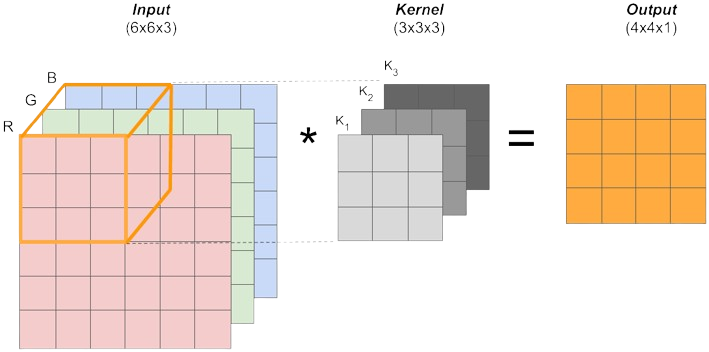
\includegraphics[width=0.9\linewidth]{Figuras/Img06.png}
\end{frame}
%%%%%%%%%%%%%%%%%%%%%%%%%%%%%%%%%%%%%%%%%%%%%%%%%%%%%%%%

%%%%%%%%%%%%%%%%%%%%%%%%%%%%%%%%%%%%%%%%%%%%%%%%%%%%%%%%
\begin{frame}
\centering
    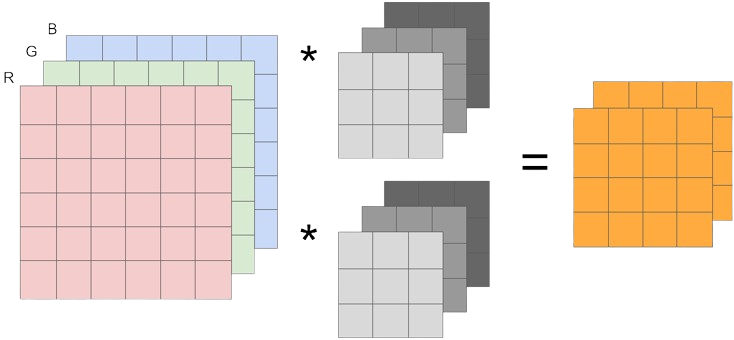
\includegraphics[width=0.9\linewidth]{Figuras/Img07.png}
\end{frame}
%%%%%%%%%%%%%%%%%%%%%%%%%%%%%%%%%%%%%%%%%%%%%%%%%%%%%%%%

%%%%%%%%%%%%%%%%%%%%%%%%%%%%%%%%%%%%%%%%%%%%%%%%%%%%%%%%
\begin{frame}
    \frametitle{Dimensiones}

    \begin{itemize}
        \item Entrada: $(n_w,n_h,n_c)$.
        \item Kernel: $(n_{k_1},n_{k_2},n_c)$.
        \item Número de kernels: $n$.
        \item Salida: 
        \[
            (n_w - n_{k_1} + 1,\ n_h - n_{k_2} + 1,\ n).
        \]
    \end{itemize}
    
\end{frame}
%%%%%%%%%%%%%%%%%%%%%%%%%%%%%%%%%%%%%%%%%%%%%%%%%%%%%%%%


%%%%%%%%%%%%%%%%%%%%%%%%%%%%%%%%%%%%%%%%%%%%%%%%%%%%%%%%
\begin{frame}
    \frametitle{Padding (Relleno)}

    Evita la reducción del tamaño de la salida agregando ceros alrededor de la entrada.

    \centering
    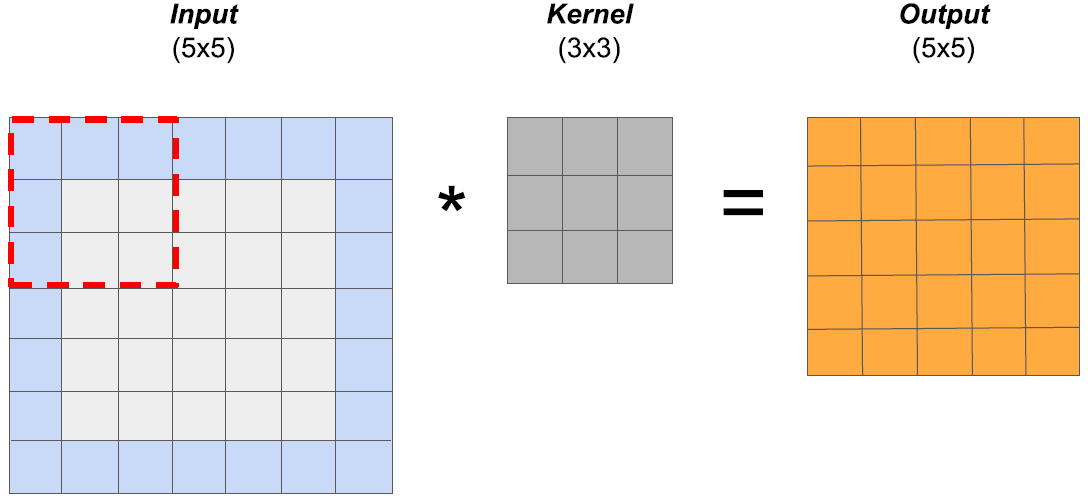
\includegraphics[width=0.67\linewidth]{Figuras/Img08.png}
\end{frame}
%%%%%%%%%%%%%%%%%%%%%%%%%%%%%%%%%%%%%%%%%%%%%%%%%%%%%%%%

%%%%%%%%%%%%%%%%%%%%%%%%%%%%%%%%%%%%%%%%%%%%%%%%%%%%%%%%
\begin{frame}
    \frametitle{Dimensiones}

    \begin{itemize}
        \item Entrada: $(n_w,n_h)$.
        \item Kernel: $(n_k,n_k)$.
        \item Valor de relleno: $p$.
        \item Salida: 
        \[
            (n_w-n_k+2p+1,\ n_h-n_k+2p+1)
        \]
    \end{itemize}

    Para mantener el tamaño de la entrada, el padding \(p\) se calcula como:
    \[
        p = \left\lfloor \frac{n_k - 1}{2} \right\rfloor
    \]
    
\end{frame}
%%%%%%%%%%%%%%%%%%%%%%%%%%%%%%%%%%%%%%%%%%%%%%%%%%%%%%%%

%%%%%%%%%%%%%%%%%%%%%%%%%%%%%%%%%%%%%%%%%%%%%%%%%%%%%%%%
\begin{frame}
    \frametitle{Convoluciones por Pasos (Stride)}

    Aplican la operación de convolución saltando celdas en la entrada.
    
    \centering
    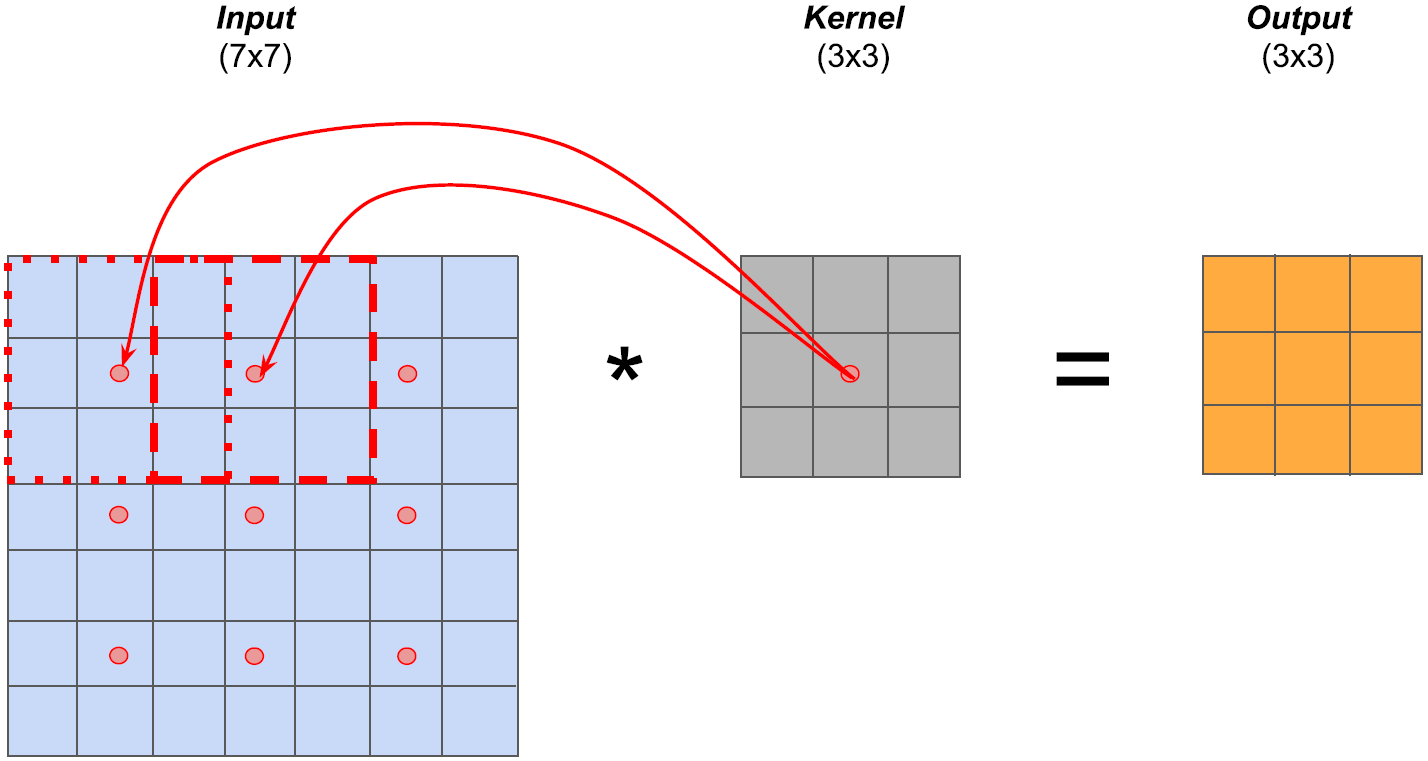
\includegraphics[width=0.67\linewidth]{Figuras/Img09.png}

\end{frame}
%%%%%%%%%%%%%%%%%%%%%%%%%%%%%%%%%%%%%%%%%%%%%%%%%%%%%%%%

%%%%%%%%%%%%%%%%%%%%%%%%%%%%%%%%%%%%%%%%%%%%%%%%%%%%%%%%
\begin{frame}
    \frametitle{Dimensiones}

    \begin{itemize}
        \item Entrada: $(n_w,n_h)$.
        \item Kernel: $(n_k,n_k)$.
        \item Valor de relleno: $p$.
        \item Paso o stride: $s$
        \item Salida: 
        \[
            \left(\left\lfloor \frac{n_w - n_k + 2p}{s} + 1 \right\rfloor ,\  \left\lfloor \frac{n_h - n_k + 2p}{s} + 1 \right\rfloor\right)
        \]
    \end{itemize}

    Reduce la dimensión de la salida al aplicar un mayor paso en la convolución.

\end{frame}
%%%%%%%%%%%%%%%%%%%%%%%%%%%%%%%%%%%%%%%%%%%%%%%%%%%%%%%%

%%%%%%%%%%%%%%%%%%%%%%%%%%%%%%%%%%%%%%%%%%%%%%%%%%%%%%%%
\begin{frame}[fragile]
    \frametitle{Capa de Agrupamiento (Pooling)}
    Reducen la dimensión de los datos de entrada.

    \begin{columns}
    \column{.5\textwidth}
    \begin{block}{Max-pooling}Valor máximo en una región de la entrada.\phantom{g}
    \end{block}
    \column{.5\textwidth}
    \begin{block}{Average-pooling}Promedio de los valores en una región.
    \end{block}
    \end{columns}

    \begin{center}
        \small
    \begin{tikzpicture}
    % Input matrix
    \matrix[matrix of math nodes,nodes={draw, minimum size=0.6cm, anchor=center, fill=celeste!40},column sep=-\pgflinewidth,row sep=-\pgflinewidth] (m1) {
        1 & 3 & 2 & 1 \\
        2 & 9 & 1 & 1 \\
        1 & 3 & 2 & 3 \\
        5 & 6 & 1 & 2 \\
    };

    % Output matrix
    \matrix[matrix of math nodes,nodes={draw, minimum size=0.6cm, anchor=center, fill=celeste!40},column sep=-\pgflinewidth,row sep=-\pgflinewidth] (m2) [right=1cm of m1] {
        9 & 2 \\
        6 & 3 \\
    };


    % Dashed boxes for pooling regions (Input)
    \draw[azul, thick, dashed] ($(m1-1-1.north west)+(-0.01,0.01)$)  rectangle ($(m1-2-2.south east)+(0.01,-0.01)$);
    \draw[purple, thick, dashed] ($(m1-1-3.north west)+(-0.01,0.01)$)  rectangle ($(m1-2-4.south east)+(0.01,-0.01)$);
    \draw[brown, thick, dashed] ($(m1-3-1.north west)+(-0.01,0.01)$)  rectangle ($(m1-4-2.south east)+(0.01,-0.01)$);
    \draw[teal, thick, dashed] ($(m1-3-3.north west)+(-0.01,0.01)$)  rectangle ($(m1-4-4.south east)+(0.01,-0.01)$);

    % Dashed boxes for pooling regions (Output)
    \draw[azul, thick, dashed] ($(m2-1-1.north west)+(-0.01,0.01)$) rectangle ($(m2-1-1.south east)+(0.01,-0.01)$);
    \draw[purple, thick, dashed] ($(m2-1-2.north west)+(-0.01,0.01)$) rectangle ($(m2-1-2.south east)+(0.01,-0.01)$);
    \draw[brown, thick, dashed] ($(m2-2-1.north west)+(-0.01,0.01)$) rectangle ($(m2-2-1.south east)+(0.01,-0.01)$);
    \draw[teal, thick, dashed] ($(m2-2-2.north west)+(-0.01,0.01)$) rectangle ($(m2-2-2.south east)+(0.01,-0.01)$);

    % Arrow from Input to Output
    \draw[->, thick] ($(m1.east)$) -- ($(m2.west)$);

    \draw[azul, thick, ->] ($(m1-1-1.north east)+(0,0.1)$) to[out=20, in=150] ($(m2-1-1.north)+(0,0.1)$);
    \end{tikzpicture}
    \end{center}
\end{frame}
%%%%%%%%%%%%%%%%%%%%%%%%%%%%%%%%%%%%%%%%%%%%%%%%%%%%%%%%

%%%%%%%%%%%%%%%%%%%%%%%%%%%%%%%%%%%%%%%%%%%%%%%%%%%%%%%%
\begin{frame}
    \frametitle{Estructura de una Red Neuronal Convolucional (CNN)}

    \begin{itemize}[leftmargin=*]
        \item \textbf{Bloque convolucional:}
        \begin{itemize}[leftmargin=*]
            \item Incluye capas de convolución, agrupamiento (pooling) y activación.
            \item Detecta patrones y características en los datos de entrada.
        \end{itemize}

        \item \textbf{Bloque totalmente conectado:}
        \begin{itemize}[leftmargin=*]
            \item Cada neurona se conecta con todas las neuronas de la capa anterior y siguiente.
            \item Correlacionan las características detectadas por las capas convolucionales.
        \end{itemize}

        \item \textbf{Bloque de decisión:}
        \begin{itemize}[leftmargin=*]
            \item Genera un vector de probabilidades para cada clase.
            \item Usa funciones como softmax.
        \end{itemize}
    \end{itemize}

\end{frame}
%%%%%%%%%%%%%%%%%%%%%%%%%%%%%%%%%%%%%%%%%%%%%%%%%%%%%%%%


%%%%%%%%%%%%%%%%%%%%%%%%%%%%%%%%%%%%%%%%%%%%%%%%%%%%%%%%
\begin{frame}[fragile]
    \frametitle{Estructura de una Red Neuronal Convolucional (CNN)}

    \begin{center}
\tikzstyle{block} = [rectangle, draw, rounded corners, minimum width=1cm, minimum height=3cm, node distance=2cm]
\begin{tikzpicture}
    % Blocks
    \node (data) {Datos};
    \node (conv) [block, right of=data, fill=green!20] {\rotatebox{90}{Bloque Convolucional}};
    \node (fc) [block, right of=conv, fill=gray!20] {\rotatebox{90}{Bloque totalmente conectado}};
    \node (softmax) [block, right of=fc, fill=red!20] {\rotatebox{90}{Bloque de decisión}};
    \node[right=of softmax] (results) {Resultados};

    % Arrows
    \draw[->] (data) -- (conv);
    \draw[->] (conv) -- (fc);
    \draw[->] (fc) -- (softmax);
    \draw[->] (softmax) -- (results);

\end{tikzpicture}
    \end{center}
\end{frame}
%%%%%%%%%%%%%%%%%%%%%%%%%%%%%%%%%%%%%%%%%%%%%%%%%%%%%%%%


%%%%%%%%%%%%%%%%%%%%%%%%%%%%%%%%%%%%%%%%%%%%%%%%%%%%%%%%
\begin{frame}[fragile]
    \frametitle{Estructura de una Red Neuronal Convolucional (CNN)}

    \begin{center}\small
\begin{tikzpicture}
    % Data block (Input)
    \node[minimum height=2.9cm, label=above:Input, minimum width=1.4cm] (data) {\rotatebox{90}{\textbf{Datos}}};
    
    % Convolutional block
    \node[draw=teal, fill=teal!10, right=0.5cm of data, minimum width=6cm, minimum height=3cm, label={[text=teal]above:Convolucional}] (convblock) {};
    
    % FC block
    \node[draw=gray, fill=gray!10, right=1cm of convblock, minimum width=1.5cm, minimum height=3cm, label={[text=gray]above:T. Conectada}] (fc) {};
    
    % Softmax block
    \node[draw=purple, fill=purple!10, right=1cm of fc, minimum width=1cm, minimum height=3cm, label={[text=purple]above:Decisión}] (softmax) {};
    
    % Convolutional layers inside convolutional block
    \node[draw=teal, minimum width=0.7cm, minimum height=2cm] (conv) at ($(convblock.west)+(0.8,0)$) {\rotatebox{90}{\color{teal}Convolución}};
    \node[draw=teal, minimum width=0.7cm, minimum height=2cm, right=0.3cm of conv] (pool) {\rotatebox{90}{\color{teal}Relleno}};
    \node[draw=teal, minimum width=0.7cm, minimum height=2cm, right=0.3cm of pool] (act) {\rotatebox{90}{\color{teal}Activación}};

    % Capa 1
    \draw[dashed, color=teal] ($(conv.west)+(-0.2,-1.3)$) rectangle ($(act.east)+(0.2,1.3)$);
    \node[below=0.5cm of pool] {\color{teal}Capa 1};
    
    % Puntos
    \node[right=0.5cm of act] (dots) {$\cdots$};

    % Capa n
    \draw[dashed, color=teal] ($(act.east)+(1.5,-1.3)$) rectangle ($(act.east)+(2.5,1.3)$);
    \node at ($(act.east)+(2,-1.8)$) {\color{teal}Capa $n$};

    % Arrow connections Convolucional
    \draw[->, thick] (data.east) -- (convblock.west);
    \draw[->, thick, teal] ($(act.east)+(0.2,0)$) -- (dots.west);
    \draw[<-, thick, teal] ($(act.east)+(1.5,0)$) -- (dots.east);

    
    % FC connections
    \node (a1) at ($(convblock.east)+(0,1)$) [inner sep=0pt]{};
    \node (a2) at ($(convblock.east)$) [inner sep=0pt]{};
    \node (a3) at ($(convblock.east)+(0,-1)$) [inner sep=0pt]{};

    \foreach \i in {-1.25,-1,...,1.25} {
        \foreach \a in {a1, a2, a3} {
            \draw[line width=0.2pt, color=gray] (\a) -- ($(fc.west)+(0.4,+\i)$);
        }
        \foreach \j in {-0.75,-0.25,...,0.75} {
            \draw[line width=0.2pt, color=gray] ($(fc.west)+(0.4,+\i)$) -- ($(fc.west)+(1.1,+\j)$);
        }
        \node at ($(fc.west)+(0.4,+\i)$) [circle, fill=gray, inner sep=1.2pt]{};
    }
    
    \foreach \j in {1,0,-1} {
        \node at ($(softmax.west)+(0.5,+\j)$) [circle, fill=purple, inner sep=1.2pt]{};
        \foreach \i in {-0.75,-0.25,...,0.75} {
            \draw[line width=0.2pt, color=purple] ($(fc.west)+(1.1,+\i)$) -- ($(softmax.west)+(0.5,+\j)$);
            \node at ($(fc.west)+(1.1,+\i)$) [circle, fill=gray, inner sep=1.2pt]{};
        }
        \draw[->, thick] ($(softmax.east)+(0,\j)$) -- ++(0.5,0);
    
    }

    % Data block (Input)
    \node[minimum height=2.9cm, minimum width=1.4cm, label=above:Output, right=0.5cm of softmax] {\rotatebox{90}{\textbf{Resultado}}};
\end{tikzpicture}
    \end{center}
\end{frame}
%%%%%%%%%%%%%%%%%%%%%%%%%%%%%%%%%%%%%%%%%%%%%%%%%%%%%%%%


%%%%%%%%%%%%%%%%%%%%%%%%%%%%%%%%%%%%%%%%%%%%%%%%%%%%%%%%
\begin{frame}
    \frametitle{Ejemplo de una CNN: LeNet-5}
    
    \centering
    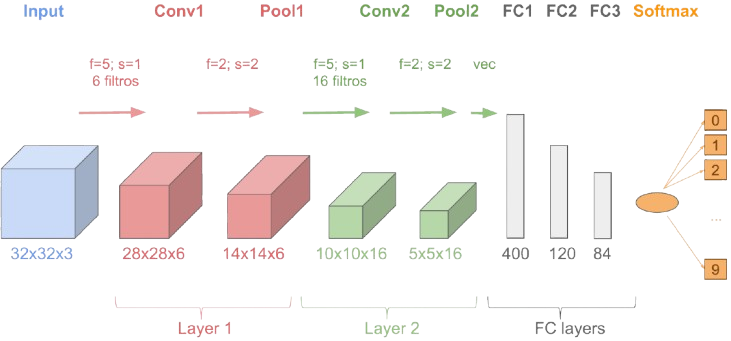
\includegraphics[width=0.9\linewidth]{Figuras/Img11.png}

\end{frame}
%%%%%%%%%%%%%%%%%%%%%%%%%%%%%%%%%%%%%%%%%%%%%%%%%%%%%%%%

%%%%%%%%%%%%%%%%%%%%%%%%%%%%%%%%%%%%%%%%%%%%%%%%%%%%%%%%
\begin{frame}
    \frametitle{Capa de Entrada (Input Layer)}
    
    \begin{itemize}
        \item La capa de entrada recibe la imagen (o los datos de entrada) y la prepara para su procesamiento.
        \item No hay parámetros que aprender en esta capa.
        \item La imagen se representa como una matriz de píxeles, que puede ser en escala de grises o RGB.
    \end{itemize}

\end{frame}
%%%%%%%%%%%%%%%%%%%%%%%%%%%%%%%%%%%%%%%%%%%%%%%%%%%%%%%%

%%%%%%%%%%%%%%%%%%%%%%%%%%%%%%%%%%%%%%%%%%%%%%%%%%%%%%%%
\begin{frame}
    \frametitle{Capas Convolucionales (Convolutional Layers)}

    \begin{itemize}
        \item Una capa convolucional tiene \( l \) canales de entrada, \( k \) canales de salida, y un tamaño de filtro \( f \).
        \item El número total de pesos es:
        \[
        f \times f \times l \times k
        \]
        \item Además, cada mapa de características tiene un valor de sesgo, por lo tanto, el número total de parámetros es:
        \[
        f \times f \times (l + 1) \times k
        \]
    \end{itemize}
    
\end{frame}
%%%%%%%%%%%%%%%%%%%%%%%%%%%%%%%%%%%%%%%%%%%%%%%%%%%%%%%%

%%%%%%%%%%%%%%%%%%%%%%%%%%%%%%%%%%%%%%%%%%%%%%%%%%%%%%%%
\begin{frame}
    \frametitle{Capas de Agrupamiento (Pooling Layers)}

    \begin{itemize}
        \item Las capas de agrupamiento (pooling) se encargan de reducir las dimensiones de las características, haciéndolas más manejables.
        \item No hay parámetros que aprender durante el proceso de entrenamiento en estas capas.
    \end{itemize}

\end{frame}
%%%%%%%%%%%%%%%%%%%%%%%%%%%%%%%%%%%%%%%%%%%%%%%%%%%%%%%%

%%%%%%%%%%%%%%%%%%%%%%%%%%%%%%%%%%%%%%%%%%%%%%%%%%%%%%%%
\begin{frame}
    \frametitle{Capas Totalmente Conectadas (Fully-Connected Layers)}

    \begin{itemize}
        \item En las capas totalmente conectadas, cada unidad de entrada se conecta con todas las unidades de salida.
        \item El número de pesos es \( n \times m \), donde \( n \) es el número de entradas y \( m \) el número de salidas.
        \item Además, cada neurona de salida tiene un valor de sesgo, por lo tanto, el número total de parámetros es:
        \[
        (n + 1) \times m
        \]
    \end{itemize}

\end{frame}
%%%%%%%%%%%%%%%%%%%%%%%%%%%%%%%%%%%%%%%%%%%%%%%%%%%%%%%%

%%%%%%%%%%%%%%%%%%%%%%%%%%%%%%%%%%%%%%%%%%%%%%%%%%%%%%%%
\begin{frame}
    \frametitle{Capa de Salida (Output Layer)}

    \begin{itemize}
        \item La capa de salida es generalmente una capa totalmente conectada.
        \item Genera las probabilidades o clasificaciones finales.
        \item El número total de parámetros en la capa de salida también es:
        \[
        (n + 1) \times m
        \]
    \end{itemize}

\end{frame}
%%%%%%%%%%%%%%%%%%%%%%%%%%%%%%%%%%%%%%%%%%%%%%%%%%%%%%%%

%%%%%%%%%%%%%%%%%%%%%%%%%%%%%%%%%%%%%%%%%%%%%%%%%%%%%%%%
\begin{frame}
    \centering
    \begin{tabular}{ccrr}
    \toprule
    \textbf{Capa}  & \textbf{Dimensión} & \textbf{Tamaño} & \textbf{Parámetros} \\ 
    \midrule
    Input   & $(32 \times 32 \times 3)$   & 3072   & 0        \\
    Conv1   & $(28 \times 28 \times 6)$   & 4704   & 456      \\ 
    Pool1   & $(14 \times 14 \times 6)$   & 1176   &         \\ 
    Conv2   & $(10 \times 10 \times 16)$  & 1600   &     \\ 
    Pool2   & $(5 \times 5 \times 16)$    & 400     &         \\ 
    FC2     & $(120 \times 1)$       & 120     &    \\ 
    FC3     & $(84 \times 1)$        & 84      &    \\ 
    Softmax & $(10 \times 1)$        & 10      &       \\ 
    \midrule
    Total &&&\\
    \bottomrule
    \end{tabular}

\end{frame}
%%%%%%%%%%%%%%%%%%%%%%%%%%%%%%%%%%%%%%%%%%%%%%%%%%%%%%%%

%%%%%%%%%%%%%%%%%%%%%%%%%%%%%%%%%%%%%%%%%%%%%%%%%%%%%%%%
\begin{frame}
    \centering
    \begin{tabular}{ccrr}
    \toprule
    \textbf{Capa}  & \textbf{Dimensión} & \textbf{Tamaño} & \textbf{Parámetros} \\ 
    \midrule
    Input   & $(32 \times 32 \times 3)$   & 3072   & 0        \\
    Conv1   & $(28 \times 28 \times 6)$   & 4704   & 456      \\ 
    Pool1   & $(14 \times 14 \times 6)$   & 1176   & 0        \\ 
    Conv2   & $(10 \times 10 \times 16)$  & 1600   & 2416    \\ 
    Pool2   & $(5 \times 5 \times 16)$    & 400     & 0        \\ 
    FC2     & $(120 \times 1)$       & 120     & 48120   \\ 
    FC3     & $(84 \times 1)$        & 84      & 10164   \\ 
    Softmax & $(10 \times 1)$        & 10      & 850      \\ 
    \midrule
    Total &&&62006\\
    \bottomrule
    \end{tabular}

\end{frame}
%%%%%%%%%%%%%%%%%%%%%%%%%%%%%%%%%%%%%%%%%%%%%%%%%%%%%%%%
